% Options for packages loaded elsewhere
\PassOptionsToPackage{unicode}{hyperref}
\PassOptionsToPackage{hyphens}{url}
%
\documentclass[
]{book}
\usepackage{lmodern}
\usepackage{amssymb,amsmath}
\usepackage{ifxetex,ifluatex}
\ifnum 0\ifxetex 1\fi\ifluatex 1\fi=0 % if pdftex
  \usepackage[T1]{fontenc}
  \usepackage[utf8]{inputenc}
  \usepackage{textcomp} % provide euro and other symbols
\else % if luatex or xetex
  \usepackage{unicode-math}
  \defaultfontfeatures{Scale=MatchLowercase}
  \defaultfontfeatures[\rmfamily]{Ligatures=TeX,Scale=1}
\fi
% Use upquote if available, for straight quotes in verbatim environments
\IfFileExists{upquote.sty}{\usepackage{upquote}}{}
\IfFileExists{microtype.sty}{% use microtype if available
  \usepackage[]{microtype}
  \UseMicrotypeSet[protrusion]{basicmath} % disable protrusion for tt fonts
}{}
\makeatletter
\@ifundefined{KOMAClassName}{% if non-KOMA class
  \IfFileExists{parskip.sty}{%
    \usepackage{parskip}
  }{% else
    \setlength{\parindent}{0pt}
    \setlength{\parskip}{6pt plus 2pt minus 1pt}}
}{% if KOMA class
  \KOMAoptions{parskip=half}}
\makeatother
\usepackage{xcolor}
\IfFileExists{xurl.sty}{\usepackage{xurl}}{} % add URL line breaks if available
\IfFileExists{bookmark.sty}{\usepackage{bookmark}}{\usepackage{hyperref}}
\hypersetup{
  pdftitle={Serious Poems for Kids},
  pdfauthor={Jiangtang Hu},
  hidelinks,
  pdfcreator={LaTeX via pandoc}}
\urlstyle{same} % disable monospaced font for URLs
\usepackage{longtable,booktabs}
% Correct order of tables after \paragraph or \subparagraph
\usepackage{etoolbox}
\makeatletter
\patchcmd\longtable{\par}{\if@noskipsec\mbox{}\fi\par}{}{}
\makeatother
% Allow footnotes in longtable head/foot
\IfFileExists{footnotehyper.sty}{\usepackage{footnotehyper}}{\usepackage{footnote}}
\makesavenoteenv{longtable}
\usepackage{graphicx,grffile}
\makeatletter
\def\maxwidth{\ifdim\Gin@nat@width>\linewidth\linewidth\else\Gin@nat@width\fi}
\def\maxheight{\ifdim\Gin@nat@height>\textheight\textheight\else\Gin@nat@height\fi}
\makeatother
% Scale images if necessary, so that they will not overflow the page
% margins by default, and it is still possible to overwrite the defaults
% using explicit options in \includegraphics[width, height, ...]{}
\setkeys{Gin}{width=\maxwidth,height=\maxheight,keepaspectratio}
% Set default figure placement to htbp
\makeatletter
\def\fps@figure{htbp}
\makeatother
\setlength{\emergencystretch}{3em} % prevent overfull lines
\providecommand{\tightlist}{%
  \setlength{\itemsep}{0pt}\setlength{\parskip}{0pt}}
\setcounter{secnumdepth}{5}
\usepackage{booktabs}
\usepackage{longtable}
\usepackage[bf,singlelinecheck=off]{caption}

\setmainfont[UprightFeatures={SmallCapsFont=AlegreyaSC-Regular}]{Alegreya}

\usepackage{framed,color}
\definecolor{shadecolor}{RGB}{248,248,248}

\renewcommand{\textfraction}{0.05}
\renewcommand{\topfraction}{0.8}
\renewcommand{\bottomfraction}{0.8}
\renewcommand{\floatpagefraction}{0.75}

\renewenvironment{quote}{\begin{VF}}{\end{VF}}
\let\oldhref\href
\renewcommand{\href}[2]{#2\footnote{\url{#1}}}

\ifxetex
  \usepackage{letltxmacro}
  \setlength{\XeTeXLinkMargin}{1pt}
  \LetLtxMacro\SavedIncludeGraphics\includegraphics
  \def\includegraphics#1#{% #1 catches optional stuff (star/opt. arg.)
    \IncludeGraphicsAux{#1}%
  }%
  \newcommand*{\IncludeGraphicsAux}[2]{%
    \XeTeXLinkBox{%
      \SavedIncludeGraphics#1{#2}%
    }%
  }%
\fi

\makeatletter
\newenvironment{kframe}{%
\medskip{}
\setlength{\fboxsep}{.8em}
 \def\at@end@of@kframe{}%
 \ifinner\ifhmode%
  \def\at@end@of@kframe{\end{minipage}}%
  \begin{minipage}{\columnwidth}%
 \fi\fi%
 \def\FrameCommand##1{\hskip\@totalleftmargin \hskip-\fboxsep
 \colorbox{shadecolor}{##1}\hskip-\fboxsep
     % There is no \\@totalrightmargin, so:
     \hskip-\linewidth \hskip-\@totalleftmargin \hskip\columnwidth}%
 \MakeFramed {\advance\hsize-\width
   \@totalleftmargin\z@ \linewidth\hsize
   \@setminipage}}%
 {\par\unskip\endMakeFramed%
 \at@end@of@kframe}
\makeatother

\renewenvironment{Shaded}{\begin{kframe}}{\end{kframe}}

\newenvironment{rmdblock}[1]
  {
  \begin{itemize}
  \renewcommand{\labelitemi}{
    \raisebox{-.7\height}[0pt][0pt]{
      {\setkeys{Gin}{width=3em,keepaspectratio}\includegraphics{images/#1}}
    }
  }
  \setlength{\fboxsep}{1em}
  \begin{kframe}
  \item
  }
  {
  \end{kframe}
  \end{itemize}
  }
\newenvironment{rmdnote}
  {\begin{rmdblock}{note}}
  {\end{rmdblock}}
\newenvironment{rmdcaution}
  {\begin{rmdblock}{caution}}
  {\end{rmdblock}}
\newenvironment{rmdimportant}
  {\begin{rmdblock}{important}}
  {\end{rmdblock}}
\newenvironment{rmdtip}
  {\begin{rmdblock}{tip}}
  {\end{rmdblock}}
\newenvironment{rmdwarning}
  {\begin{rmdblock}{warning}}
  {\end{rmdblock}}

\usepackage{makeidx}
\makeindex

\urlstyle{tt}

\usepackage{amsthm}
\makeatletter
\def\thm@space@setup{%
  \thm@preskip=8pt plus 2pt minus 4pt
  \thm@postskip=\thm@preskip
}
\makeatother

\frontmatter
\usepackage[]{natbib}
\bibliographystyle{plainnat}

\title{Serious Poems for Kids}
\author{Jiangtang Hu}
\date{2019-09-19}

\begin{document}
\frontmatter
\maketitle

%\cleardoublepage\newpage\thispagestyle{empty}\null
%\cleardoublepage\newpage\thispagestyle{empty}\null
%\cleardoublepage\newpage
\thispagestyle{empty}
\begin{center}
\includegraphics{images/dedication.pdf}
\end{center}

\setlength{\abovedisplayskip}{-5pt}
\setlength{\abovedisplayshortskip}{-5pt}

{
\setcounter{tocdepth}{2}
\tableofcontents
}
\mainmatter
\hypertarget{section}{%
\chapter*{}\label{section}}
\addcontentsline{toc}{chapter}{}

\url{http://jiangtanghu.com/4you}

Kids can appreciate William Carlos Williams' Red Wheelbarrow, even it was not necessary written for kids.

For this purpose, this collection excludes the wonderful poems from Shel Silverstein, Edward Lear and such.).

```

\hypertarget{section-1}{%
\chapter{诗经}\label{section-1}}

\hypertarget{section-2}{%
\section{大雅:大明}\label{section-2}}

\begin{quote}
明明在下,\\
赫赫在上。
\end{quote}

\includegraphics{images/.jpg}

\hypertarget{section-3}{%
\chapter{论语}\label{section-3}}

\hypertarget{section-4}{%
\section{乡党:厩焚}\label{section-4}}

\begin{quote}
厩焚,\\
子退朝,曰:\\
伤人乎?\\
不问马。
\end{quote}

\hypertarget{section-5}{%
\section{先进:侍坐}\label{section-5}}

\begin{quote}
暮春者,\\
春服既成,\\
冠者五六人,\\
童子六七人,\\
浴乎沂,\\
风乎舞雩,\\
咏而归。
\end{quote}

\hypertarget{section-6}{%
\chapter{苏轼}\label{section-6}}

\hypertarget{section-7}{%
\section{记承天寺夜游}\label{section-7}}

\begin{quote}
元丰六年十月十二日夜,\\
解衣欲睡,\\
月色入户,\\
欣然起行。

念无与为乐者,\\
遂至承天寺寻张怀民。\\
怀民亦未寝,\\
相与步于中庭。

庭下如积水空明,\\
水中藻荇交横,\\
盖竹柏影也。

何夜无月?\\
何处无竹柏?\\
但少闲人如吾两人者耳。
\end{quote}

\hypertarget{section-8}{%
\chapter{张岱}\label{section-8}}

\hypertarget{section-9}{%
\section{湖心亭看雪}\label{section-9}}

\begin{quote}
崇祯五年十二月,\\
余住西湖。\\
大雪三日,\\
湖中人鸟声俱绝。

是日更定矣,\\
余挐一小舟,\\
拥毳衣炉火,\\
独往湖心亭看雪。

雾凇沆砀,\\
天与云与山与水,\\
上下一白。\\
湖上影子,\\
惟长堤一痕、\\
湖心亭一点、\\
与余舟一芥,\\
舟中人两三粒而已。

到亭上,\\
有两人铺毡对坐,\\
一童子烧酒,\\
炉正沸。\\
见余大喜,曰:\\
``湖中焉得更有此人!''\\
拉余同饮。

余强饮三大白而别。\\
问其姓氏,\\
是金陵人,\\
客此。

及下船,\\
舟子喃喃曰:\\
``莫说相公痴,\\
更有痴似相公者!''
\end{quote}

\hypertarget{section-10}{%
\chapter{钱镠}\label{section-10}}

\hypertarget{section-11}{%
\section{陌上花开}\label{section-11}}

\begin{quote}
陌上花开,\\
可缓缓归矣。
\end{quote}

\includegraphics{images/.jpg}

\hypertarget{section-12}{%
\chapter{丘迟}\label{section-12}}

\hypertarget{section-13}{%
\section{与陈伯之书}\label{section-13}}

\begin{quote}
暮春三月,\\
江南草长,\\
杂花生树,\\
群莺乱飞。
\end{quote}

\includegraphics{images/.jpg}

\hypertarget{section-14}{%
\chapter{卞之琳}\label{section-14}}

\hypertarget{section-15}{%
\section{断章}\label{section-15}}

\begin{quote}
你站在桥上看风景,\\
看风景的人在楼上看你。\\
明月装饰了你的窗子,\\
你装饰了别人的梦。
\end{quote}

\includegraphics{images/.jpg}

\hypertarget{section-16}{%
\chapter{江河}\label{section-16}}

\hypertarget{section-17}{%
\section{让我们一起奔腾吧之一}\label{section-17}}

\begin{quote}
我和春天一起写这首诗\\
和你和更多的人一同唱这支歌\\
海水和冰块猛烈相撞。船冲向浪头\\
我们这样站着,雄壮而多情\\
温柔地呼唤风象召唤姑娘们\\
使大地上所有的树木都涨满绿帆\\
当喷吐着鲜红火焰的果子\\
被狂风一个个击落,那时候\\
种子就撒遍土地,和矿藏---同沉默着\\
为了在今天歌唱\\
让我们一块儿走吧\\
为了歌唱,玉兰花\\
洁白的心向蓝天打开\\
为了不再孤独,繁星似的迎春到处闪烁\\
金色的声音刺激着我们\\
阳光追逐着,鸟儿牵动着\\
让我们一块儿走吧\\
在花瓣匆匆铺就的道路上芬芳地走吧\\
紫丁香象影子一样在身后晃动\\
五月正迎着我们走来,献上更多的花朵
\end{quote}

\hypertarget{section-18}{%
\section{让我们一起奔腾吧之二}\label{section-18}}

\begin{quote}
你热情,开朗,象四月的阳光\\
想象的云朵在疾风中飞扬\\
寻找美好的声音\\
爱情的震颤,庄稼的波涛,金属的鸣响\\
走向辽远的地方,放出喉咙里的力量\\
你一阵又一阵风似地跑来\\
告诉我使你坐不住的事情\\
捧着激荡的诗\\
一直读到希望战栗着升起\\
抖索黎明时分蓝色的锋芒\\
我知道你善良的愿望,你所原谅的姑娘\\
你原谅的生活中渐渐迷茫的目光\\
但那不能原谅的一切\\
尖锐地刺痛你\\
你僧恨黑暗,甚至阴影\\
因此清澈地对待别人,清澈得\\
看到了心,一颗浆果在绿叶丛中摇荡\\
你将一年又一年把这鲜红的果子挂满枝头\\
让善良的人们摘去\\
想到你,我的诗中就扬起好听的声响
\end{quote}

\hypertarget{section-19}{%
\section{让我们一起奔腾吧之三}\label{section-19}}

\begin{quote}
我们结识了,岩石\\
用大海翡翠的语言交谈\\
用坦白得象沙滩一样的语言\\
雪花似的水鸟栖息在我们的肩头\\
飞去又回来,我们就这样和天空对话\\
我们结识了。江河\\
蔚蓝地在黑土地上流过\\
太阳和星星睡在我们的怀里\\
闪闪发光,颤动着金碧辉煌的梦\\
点点白帆象纯洁的姑娘们伴随着我们

山上长满倔强的针叶树\\
在冬天也是绿色的战士
\end{quote}

\hypertarget{section-20}{%
\section{让我们一起奔腾吧之四}\label{section-20}}

\begin{quote}
让我们一块儿走吧\\
土地说:我要接近天空\\
于是,山脉耸起\\
人说:我要生活\\
于是,洪水退去\\
河流优美地流着\\
让我们和更多的人一块儿走吧\\
祖先在风中诉说着青葱的愿望\\
血液在身体里温暖地流着,在太阳上欢跃\\
太阳把七色的花朵投在成千上万的枝条上\\
我们又将给大地留下什么\\
成千上万只叶子的小船从枝条出发\\
大海把清脆的浪花投进岩石缝中\\
我们的手臂又将收获什么\\
岁月的皱纹又将闪出什么样的光辉\\
我不能设想,美丽的风光\\
不在人们脸上闪动\\
我们死去和诞生的地方还有什么意义\\
我不能设想,崛起的建筑\\
不溢满普通家庭的笑声\\
我们的劳动、创造还有什么意义\\
为此\\
我和大海一同醒来,拿起工具\\
春天伴随着我们一块儿走来
\end{quote}

\includegraphics{images/.jpg}

\hypertarget{section-21}{%
\chapter{海子}\label{section-21}}

\hypertarget{section-22}{%
\section{面朝大海,春暖花开}\label{section-22}}

\begin{quote}
从明天起,做一个幸福的人\\
喂马,劈柴,周游世界\\
从明天起,关心粮食和蔬菜\\
我有一所房子,面朝大海,春暖花开

从明天起,和每一个亲人通信\\
告诉他们我的幸福\\
那幸福的闪电告诉我的\\
我将告诉每一个人\\
给每一条河每一座山取一个温暖的名字

陌生人,我也为你祝福\\
愿你有一个灿烂的前程\\
愿你有情人终成眷属\\
愿你在尘世获得幸福\\
我只愿面朝大海,春暖花开
\end{quote}

\hypertarget{s}{%
\section{献诗------给S}\label{s}}

\begin{quote}
谁在美丽的早晨
谁在这一首诗中

谁在美丽的火中飞行
并给与我无限的赠予

谁在炊烟散尽的村庄
谁在晴朗的高空

天上的白云
是谁的伴侣

谁身体黑如夜晚 两翼雪白
在思念 在鸣叫

谁在美丽的早晨
谁在这一首诗中
\end{quote}

\hypertarget{section-23}{%
\section{活在这珍贵的人间}\label{section-23}}

\begin{quote}
活在这珍贵的人间\\
太阳强烈\\
水波温柔\\
一层层白云覆盖着
我\\
踩在青草上\\
感到自己是彻底干净的黑土块

活在这珍贵的人间\\
泥土高溅\\
扑打面颊\\
活在这珍贵的人间\\
人类和植物一样幸福\\
爱情和雨水一样幸福
\end{quote}

\hypertarget{section-24}{%
\section{我无限的热爱着新的一日}\label{section-24}}

\begin{quote}
我无限的热爱着新的一日\\
今天的太阳今天的马今天的花楸树\\
使我健康富足拥有一生

从黎明到黄昏\\
阳光充足\\
胜过一切过去的诗\\
幸福找到我\\
幸福说:``瞧这个诗人\\
他比我本人还要幸福''

在劈开了我的秋天\\
在劈开了我的骨头的秋天\\
我爱你,花楸树
\end{quote}

\hypertarget{section-25}{%
\chapter{鲁迅}\label{section-25}}

\hypertarget{section-26}{%
\section{答客诮}\label{section-26}}

\begin{quote}
无情未必真豪杰,\\
怜子如何不丈夫?\\
知否兴风狂啸者,\\
回眸时看小於菟?
\end{quote}

\includegraphics{images/.jpg}

\hypertarget{section-27}{%
\chapter{黄灿然}\label{section-27}}

\hypertarget{section-28}{%
\section{献给妻子}\label{section-28}}

\begin{quote}
很久了,我没有为你写诗,\\
你曾是我灵感的唯一源泉;\\
在我这久经风浪的心底\\
仍时常激荡着我们的初恋;

但是我的心实在是衰老了,\\
因为它过早地遇到了风暴\\
并从多次的险境中逃脱,\\
我怎能不抒发这种逼迫?

如今我在异乡艰苦劳动,\\
为了让你的双手与众不同:\\
以前没有受过磨难,以后

也将永远闲置在安适之中:\\
繁重的工作就是我的情诗,\\
所有的成果全部献给你。
\end{quote}

\includegraphics{images/.jpg}

\hypertarget{section-29}{%
\chapter{李元胜}\label{section-29}}

\hypertarget{section-30}{%
\section{我想和你虚度时光,比如低头看鱼}\label{section-30}}

\begin{quote}
我想和你虚度时光,比如低头看鱼
比如把茶杯留在桌子上,离开
浪费它们好看的阴影

我还想连落日一起浪费,比如散步
一直消磨到星光满天
我还要浪费风起的时候
坐在走廊发呆,直到你眼中乌云
全部被吹到窗外
我已经虚度了世界,它经过我
疲倦,又像从未被爱过
但是明天我还要这样,虚度
满目的花草,生活应该像它们一样美好
一样无意义,像被虚度的电影
那些绝望的爱和赴死
为我们带来短暂的沉默
我想和你互相浪费
一起虚度短的沉默,长的无意义
一起消磨精致而苍老的宇宙
比如靠在栏杆上,低头看水的镜子
直到所有被虚度的事物
在我们身后,长出薄薄的翅膀
\end{quote}

\hypertarget{section-31}{%
\chapter{泰戈尔}\label{section-31}}

\hypertarget{section-32}{%
\section{新月集:职业}\label{section-32}}

\begin{quote}
早晨,钟敲十下的时候,我沿着我们的小巷到学校去。\\
每天我都遇见那个小贩,他叫道:``镯子呀,亮晶晶的镯子!''\\
他没有什么事情急着要做,他没有哪条街一定要走,他没有什么地方一定要去,他没有什么时间一定要回家。\\
我愿意我是一个小贩,在街上过日子,叫着:``镯子呀,亮晶晶的镯子!''

下午四点,我从学校里回家。\\
从一家门口,我看得见一个园丁在那里掘地。\\
他用他的锄子,要怎么掘,便怎么掘,他被尘土污了衣裳,如果他被太阳晒黑了或是身上被打湿了,都没有人骂他。\\
我愿意我是一个园丁,在花园里掘地。 谁也不来阻止我。

天色刚黑,妈妈就送我上床。\\
从开着的窗口,我看得见更夫走来走去。\\
小巷又黑又冷清,路灯立在那里,像一个头上生着一只红眼睛的巨人。\\
更夫摇着他的提灯,跟他身边的影子一起走着,他一生一次都没有上床去过。\\
我愿意我是一个更夫,整夜在街上走,提了灯去追逐影子。
\end{quote}

\hypertarget{section-33}{%
\section{新月集:家庭}\label{section-33}}

\begin{quote}
我独自在横跨过田地的路上走着,\\
夕阳像一个守财奴似的,\\
正藏起它的最后的金子。

白昼更加深沉地投入黑暗之中,\\
那已经收割了的孤寂的田地,\\
默默地躺在那里。

天空里突然升起了一个男孩子的尖锐的歌声。\\
他穿过看不见的黑暗,\\
留下他的歌声的辙痕跨过黄昏的静谧。

他的乡村的家坐落在荒凉的边上,\\
在甘蔗田的后面,\\
躲藏在香蕉树,\\
瘦长的槟榔树,\\
椰子树和深绿色的贾克果树的阴影里。

我在星光下独自走着的路上停留了一会,\\
我看见黑沉沉的大地展开在我的面前,\\
用她的手臂拥抱着无量数的家庭,\\
在那些家庭里有着摇篮和床铺,\\
母亲们的心和夜晚的灯,\\
还有年轻轻的生命,\\
他们满心欢乐,\\
却浑然不知这样的欢乐对于世界的价值。
\end{quote}

\hypertarget{section-34}{%
\section{新月集:孩童之道}\label{section-34}}

\begin{quote}
只要孩子愿意,他此刻便可飞上天去。\\
他所以不离开我们,并不是没有缘故。\\
他爱把他的头倚在妈妈的胸间,他即使是一刻不见她,也是不行的。\\
孩子知道各式各样的聪明话,虽然世间的人很少懂得这些话的意义。\\
他所以永不想说,并不是没有缘故。

他所要做的一件事,就是要学习从妈妈的嘴唇里说出来的话。 那就是他所以看来这样天真的缘故。\\
孩子有成堆的黄金与珠子,但他到这个世界上来,却像一个乞丐。\\
他所以这样假装了来,并不是没有缘故。

这个可爱的小小的裸着身体的乞丐,所以假装着完全无助的样子,便是想要乞求妈妈的爱的财富。\\
孩子在纤小的新月的世界里,是一切束缚都没有的。\\
他所以放弃了他的自由,并不是没有缘故。

他知道有无穷的快乐藏在妈妈的心的小小一隅里,被妈妈亲爱的手臂所拥抱,其甜美远胜过自由。\\
孩子永不知道如何哭泣。 他所住的是完全的乐土。\\
他所以要流泪,并不是没有缘故。\\
虽然他用了可爱的脸儿上的微笑,引逗得他妈妈的热切的心向着他,然而他的因为细故而发的小小的哭声,却编成了怜与爱的双重约束的带子。
\end{quote}

\hypertarget{section-35}{%
\section{新月集:小大人}\label{section-35}}

\begin{quote}
我人很小,因为我是一个小孩子,到了我像爸爸一样年纪时,便要变大了。\\
我的先生要是走来说道:``时候晚了,把你的石板,你的书拿来。''\\
我便要告诉他道:``你不知道我已经同爸爸一样大了么?\\
我决不再学什么功课了。''\\
我的老师便将惊异地说道:``他读书不读书可以随便,因为他是大人了。''

我将自己穿了衣裳,走到人群拥挤的市场里去。\\
我的叔叔要是跑过来说道:``你要迷路了,我的孩子,让我领着你罢。''\\
我便要回答道:``你没有看见么,叔叔,我已经同爸爸一样大了? 我决定要独自一个人到市场里去。''\\
叔叔便将说道:``是的,他随便到哪里去都可以,因为他是大人了。''

当我正拿钱给我保姆时,妈妈便要从浴室中出来,因为我是知道怎样用我的钥匙去开银箱的。\\
妈妈要是说道:``你在做什么呀,顽皮的孩子?''\\
我便要告诉她道:``妈妈,你不知道我已经同爸爸一样大了么? 我必须拿钱给保姆。''\\
妈妈便将自言自语道:``他可以随便把钱给他所喜欢的人,因为他是大人了。''

当十月里放假的时候,爸爸将要回家,他会以为我还是一个小孩子,为我从城里带了小鞋子和小绸衫来。\\
我便要说道:``爸爸,把这些东西给哥哥罢,因为我已经同你一样大了。''\\
爸爸便将想了一想,说道;``他可以随便去买他自己穿的衣裳,因为他是大人了。''
\end{quote}

\hypertarget{section-36}{%
\section{新月集:英雄}\label{section-36}}

\begin{quote}
妈妈,让我们想象我们正在旅行,经过一个陌生而危险的国土。\\
你坐在一顶轿子里,我骑着一匹红马,在你旁边跑着。\\
是黄昏的时候,太阳已经下山了。 约拉地希的荒地疲乏而灰暗地展开在我们面前,大地是凄凉而荒芜的。\\
你害怕了,想道------``我不知道我们到了什么地方了。''\\
我对你说道:``妈妈,不要害怕。''

草地上刺蓬蓬地长着针尖似的草,一条狭而崎岖的小道通过这块草地。\\
在这片广大的地面上看不见一只牛;它们已经回到它们村里的牛棚去了。\\
天色黑了下来,大地和天空都显得朦朦胧胧的,而我们不能说出我们正走向什么所在。

突然间,你叫我,悄悄地问我道:``靠近河岸的是什么火光呀?''\\
正在那个时候,一阵可怕的吶喊声爆发了,好些人影子向我们跑过来。\\
你蹲坐在你的轿子里,嘴里反复地祷念着神的名字。\\
轿夫们,怕得发抖,躲藏在荆棘丛中。

我向你喊道:``不要害怕,妈妈,有我在这里。''\\
他们手里执着长棒,头发披散着,越走越近了。\\
我喊道:``要当心! 你们这些坏蛋! 再向前走一步,你们就要送命了。''\\
他们又发出一阵可怕的吶喊声,向前冲过来。

你抓住我的手,说道:``好孩子,看在上天面上,躲开他们罢。''\\
我说道:``妈妈,你瞧我的。''\\
于是我刺策着我的马匹,猛奔过去,我的剑和盾彼此碰著作响。

这一场战斗是那么激烈,妈妈,如果你从轿子里看得见的话,你一定会发冷战的。\\
他们之中,许多人逃走了,还有好些人被砍杀了。\\
我知道你那时独自坐在那里,心里正在想着,你的孩子这时候一定已经死了。

但是我跑到你的跟前,浑身溅满了鲜血,说道:``妈妈,现在战争已经结束了。''\\
你从轿子里走出来,吻着我,把我搂在你的心头,你自言自语地说道:\\
``如果我没有我的孩子护送我,我简直不知道怎么办才好。''

一千件无聊的事天天在发生,为什么这样一件事不能够偶然实现呢?\\
这很像一本书里的一个故事。\\
我的哥哥要说道:``这是可能的事么? 我老是在想,他是那么嫩弱呢!''\\
我们村里的人们都要惊讶地说道:``这孩子正和他妈妈在一起,这不是很幸运么?''
\end{quote}

\hypertarget{section-37}{%
\section{新月集:责备}\label{section-37}}

\begin{quote}
为什么你眼里有了眼泪,我的孩子?\\
他们真是可怕,常常无谓地责备你!\\
你写字时墨水玷污了你的手和脸------这就是他们所以骂你龌龊的缘故么?\\
呵,呸! 他们也敢因为圆圆的月儿用墨水涂了脸,便骂它龌龊么?\\
他们总要为了每一件小事去责备你,我的孩子。 他们总是无谓地寻人错处。\\
你游戏时扯破了你的衣服------这就是他们说你不整洁的缘故么?\\
呵,呸! 秋之晨从它的破碎的云衣中露出微笑。 那末,他们要叫它什么呢?\\
他们对你说什么话,尽管可以不去理睬他,我的孩子。\\
他们把你做错的事长长地记了一笔帐。\\
谁都知道你是十分喜欢糖果的------这就是他们所以称你做贪婪的缘故么?\\
呵,呸! 我们是喜欢你的,那末,他们要叫我们什么呢?
\end{quote}

\hypertarget{section-38}{%
\section{新月集:玩具}\label{section-38}}

\begin{quote}
孩子,你真是快活呀,一早晨坐在泥土里,耍着折下来的小树枝儿。\\
我微笑地看你在那里耍着那根折下来的小树枝儿。\\
我正忙着算账,一小时一小时在那里加迭数字。\\
也许你在看我,想道:这种好没趣的游戏,竟把你的一早晨的好时间浪费掉了!\\
孩子,我忘了聚精会神玩耍树枝与泥饼的方法了。\\
我寻求贵重的玩具,收集金块与银块。\\
你呢,无论找到什么便去做你的快乐的游戏,我呢,却把我的时间与力气都浪费在那些我永不能得到的东西上。\\
我在我的脆薄的独木船里挣扎着要航过欲望之海,意忘了我也是在那里做游戏了。
\end{quote}

\hypertarget{section-39}{%
\section{新月集:天文家}\label{section-39}}

\begin{quote}
我不过说:``当傍晚圆圆的满月挂在迦昙波1的枝头时,有人能去捉住它么?''\\
哥哥却对我笑道:``孩子呀,你真是我所见到的顶顶傻的孩子。 月亮离我们这样远,谁能去捉住它呢?''\\
我说:``哥哥,你真傻! 当妈妈向窗外探望,微笑着往下看我们游戏时,你也能说她远么?''\\
哥哥还是说:``你这个傻孩子! 但是,孩子,你到哪里去找一个大得能逮住月亮的网呢?''

我说:``你自然可以用双手去捉住它呀。''\\
但是哥哥还是笑着说:``你真是我所见到的顶顶傻的孩子! 如果月亮走近了,你便知道它是多么大了。''\\
我说:``哥哥,你们学校里所教的,真是没有用呀! 当妈妈低下脸儿跟我们亲嘴时,她的脸看来也是很大的么?''\\
但是哥哥还是说:``你真是一个傻孩子。''
\end{quote}

\hypertarget{section-40}{%
\section{新月集:金色花}\label{section-40}}

\begin{quote}
假如我变了一朵金色花1,只是为了好玩,长在那棵树的高枝上,笑哈哈地在风中摇摆,又在新生的树叶上跳舞,妈妈,你会认识我么?\\
你要是叫道:``孩子,你在哪里呀?''我暗暗地在那里匿笑,却一声儿不响。\\
我要悄悄地开放花瓣儿,看着你工作。\\
当你沐浴后,湿发披在两肩,穿过金色花的林荫,走到你做祷告的小庭院时,你会嗅到这花的香气,却不知道这香气是从我身上来的。\\
当你吃过中饭,坐在窗前读《罗摩衍那》2,那棵树的阴影落在你的头发与膝上时,我便要投我的小小的影子在你的书页上,正投在你所读的地方。\\
但是你会猜得出这就是你的小孩子的小影子么?\\
当你黄昏时拿了灯到牛棚里去,我便要突然地再落到地上来,又成了你的孩子,求你讲个故事给我听。\\
``你到哪里去了,你这坏孩子?''\\
``我不告诉你,妈妈。''这就是你同我那时所要说的话了。
\end{quote}

\hypertarget{section-41}{%
\section{新月集:仙人世界}\label{section-41}}

\begin{quote}
如果人们知道了我的国王的宫殿在哪里,它就会消失在空气中的。\\
墙壁是白色的银,屋顶是耀眼的黄金。\\
皇后住在有七个庭院的宫苑里;她戴的一串珠宝,值得整整七个王国的全部财富。\\
不过,让我悄悄地告诉你,妈妈,我的国王的宫殿究竟在哪里。\\
它就在我们阳台的角上,在那栽着杜尔茜花的花盆放着的地方。\\
公主躺在远远的隔着七个不可逾越的重洋的那一岸沉睡着。\\
除了我自己,世界上便没有人能够找到她。\\
她臂上有镯子,她耳上挂着珍珠;她的头发拖到地板上。\\
当我用我的魔杖点触她的时候,她就会醒过来,而当她微笑时,珠玉将会从她唇边落下来。\\
不过,让我在我的耳朵边悄悄地告诉你,妈妈;她就住在我们阳台的角上,在那栽着杜尔茜花的花盆放着的地方。\\
当你要到河里洗澡的时候,你走上屋顶的那座阳台来罢。\\
我就坐在墙的阴影所聚会的一个角落里。\\
我只让小猫儿跟我在一起,因为它知道那故事里的理发匠住的地方。\\
不过,让我在你的耳朵边悄悄地告诉你,那故事里的理发匠到底住在哪里。\\
他住的地方,就在阳台的角上,在那栽着杜尔茜花的花盆放着的地方。
\end{quote}

\hypertarget{section-42}{%
\section{新月集:纸船}\label{section-42}}

\begin{quote}
我每天把纸船一个个放在急流的溪中。\\
我用大黑字写我的名字和我住的村名在纸船上。\\
我希望住在异地的人会得到这纸船,知道我是谁。\\
我把园中长的秀利花载在我的小船上,希望这些黎明开的花能在夜里被平平安安地带到岸上。\\
我投我的纸船到水里,仰望天空,看见小朵的云正张着满鼓着风的白帆。\\
我不知道天上有我的什么游伴把这些船放下来同我的船比赛! 夜来了,我的脸埋在手臂里,梦见我的纸船在子夜的星光下缓缓地浮泛前去。\\
睡仙坐在船里,带着满载着梦的篮子。
\end{quote}

\hypertarget{section-43}{%
\section{新月集:水手}\label{section-43}}

\begin{quote}
船夫曼特胡的船只停泊在拉琪根琪码头。\\
这只船无用地装载着黄麻,无所事事地停泊在那里已经好久了。\\
只要他肯把他的船借给我,我就给它安装一百只桨,扬起五个或六个或七个布帆来。\\
我决不把它驾驶到愚蠢的市场上去。\\
我将航行遍仙人世界里的七个大海和十三条河道。\\
但是,妈妈,你不要躲在角落里为我哭泣。\\
我不会像罗摩犍陀罗1似的,到森林中去,一去十四年才回来。\\
我将成为故事中的王子,把我的船装满了我所喜欢的东西。\\
我将带我的朋友阿细和我作伴,我们要快快乐乐地航行于仙人世界里的七个大海和十三条河道。\\
我将在绝早的晨光里张帆航行。\\
中午,你正在池塘里洗澡的时候,我们将在一个陌生的国王的国土上了。\\
我们将经过特浦尼浅滩,把特潘塔沙漠抛落在我们的后边。\\
当我们回来的时候,天色快黑了,我将告诉你我们所见到的一切。\\
我将越过仙人世界里的七个大海和十三条河道。
\end{quote}

\hypertarget{section-44}{%
\section{新月集:对岸}\label{section-44}}

\begin{quote}
我渴想到河的对岸去。\\
在那边,好些船只一行儿系在竹杆上;\\
人们在早晨乘船渡过那边去,肩上扛着犁头,去耕耘他们的远处的田;\\
在那边,牧人使他们鸣叫着的牛游泳到河旁的牧场去;\\
黄昏的时候,他们都回家了,只留下豺狼在这满长着野草的岛上哀叫。\\
妈妈,如果你不在意,我长大的时候,要做这渡船的船夫。\\
据说有好些古怪的池塘藏在这个高岸之后。\\
雨过去了,一群一群的野鹜飞到那里去,茂盛的芦苇在岸边四围生长,水鸟在那里生蛋;\\
竹鸡带着跳舞的尾巴,将它们细小的足印印在洁净的软泥上;\\
黄昏的时候,长草顶着白花,邀月光在长草的波浪上浮游。\\
妈妈,如果你不在意,我长大的时候,要做这渡船的船夫。\\
我要自此岸至彼岸,渡过来,渡过去,所有村中正在那儿沐浴的男孩女孩,都要诧异地望着我。\\
太阳升到中天,早晨变为正午了,我将跑到你那里去,说道:``妈妈,我饿了!''\\
一天完了,影子俯伏在树底下,我便要在黄昏中回家来。\\
我将永不同爸爸那样,离开你到城里去作事。\\
妈妈,如果你不在意,我长大的时候,要做这渡船的船夫。
\end{quote}

\hypertarget{section-45}{%
\section{新月集:花的学校}\label{section-45}}

\begin{quote}
当雷云在天上轰响,六月的阵雨落下的时候,\\
润湿的东风走过荒野,在竹林中吹着口笛。\\
于是一群一群的花从无人知道的地方突然跑出来,在绿草上狂欢地跳着舞。\\
妈妈,我真的觉得那群花朵是在地下的学校里上学。\\
他们关了门做功课,如果他们想在散学以前出来游戏,他们的老师是要罚他们站壁角的。\\
雨一来,他们便放假了。\\
树枝在林中互相碰触着,绿叶在狂风里萧萧地响着,雷云拍着大手,花孩子们便在那时候穿了紫的、黄的、白的衣裳,冲了出来。\\
你可知道,妈妈,他们的家是在天上,在星星所住的地方。\\
你没有看见他们怎样地急着要到那儿去么? 你不知道他们为什么那样急急忙忙么?\\
我自然能够猜得出他们是对谁扬起双臂来:他们也有他们的妈妈,就像我有我自己的妈妈一样。
\end{quote}

\hypertarget{section-46}{%
\section{新月集:商人}\label{section-46}}

\begin{quote}
妈妈,让我们想象,你待在家里,我到异邦去旅行。\\
再想象,我的船已经装得满满地在码头上等候启碇了。\\
现在,妈妈,好生想一想再告诉我,回来的时候我要带些什么给你。\\
妈妈,你要一堆一堆的黄金么?\\
在金河的两岸,田野里全是金色的稻实。\\
在林荫的路上,金色花也一朵一朵地落在地上。\\
我要为你把它们全都收拾起来,放在好几百个篮子里。\\
妈妈,你要秋天的雨点一般大的珍珠么?\\
我要渡海到珍珠岛的岸上去。\\
那个地方,在清晨的曙光里,珠子在草地的野花上颤动,珠子落在绿草上,珠子被汹狂的海浪一大把一大把地撒在沙滩上。\\
我的哥哥呢,我要送他一对有翼的马,会在云端飞翔的。\\
爸爸呢,我要带一支有魔力的笔给他,他还没有觉得,笔就写出字来了。\\
你呢,妈妈,我一定要把那个值七个王国的首饰箱和珠宝送给你。
\end{quote}

\hypertarget{section-47}{%
\section{新月集:同情}\label{section-47}}

\begin{quote}
如果我只是一只小狗,而不是你的小孩,亲爱的妈妈,当我想吃你的盘里的东西时,你要向我说``不''么?\\
你要赶开我,对我说道:``滚开,你这淘气的小狗''么?\\
那末,走罢,妈妈,走罢! 当你叫唤我的时候,我就永不到你那里去,也永不要你再喂我吃东西了。

如果我只是一只绿色的小鹦鹉,而不是你的小孩,亲爱的妈妈,你要把我紧紧地锁住,怕我飞走么?\\
你要对我摇你的手,说道:``怎样的一个不知感恩的贱鸟呀! 整夜地尽在咬它的链子''么?\\
那末,走罢,妈妈,走罢! 我要跑到树林里去;我就永不再让你抱我在你的臂里了。
\end{quote}

\hypertarget{section-48}{%
\section{新月集:长者}\label{section-48}}

\begin{quote}
妈妈,你的孩子真傻! 她是那末可笑地不懂得事!\\
她不知道路灯和星星的分别。\\
当我们玩着把小石子当食物的游戏时,她便以为它们真是吃的东西,竟想放进嘴里去。\\
当我翻开一本书,放在她面前,在她读a,b,c时,她却用手把书页撕了,无端快活地叫起来,你的孩子就是这样做功课的。\\
当我生气地对她摇头,骂她,说她顽皮时,她却哈哈大笑,以为很有趣。\\
谁都知道爸爸不在家,但是,如果我在游戏时高声叫一声``爸爸'',她便要高兴地四面张望,以为爸爸真是近在身边。\\
当我把洗衣人带来载衣服回去的驴子当做学生,并且警告她说,我是老师,她却无缘无故地乱叫起我哥哥来。\\
你的孩子要捉月亮。\\
她是这样的可笑;她把格尼许1唤作琪奴许。\\
妈妈,你的孩子真傻,她是那末可笑地不懂事!
\end{quote}

\hypertarget{section-49}{%
\section{新月集:著作家}\label{section-49}}

\begin{quote}
你说爸爸写了许多书,但我却不懂得他所写的东西。\\
他整个黄昏读书给你听,但是你真懂得他的意思么?\\
妈妈,你给我们讲的故事,真是好听呀! 我很奇怪,爸爸为什么不能写那样的书呢?\\
难道他从来没有从他自己的妈妈那里听见过巨人和神仙和公主的故事么?\\
还是已经完全忘记了?\\
他常常耽误了沐浴,你不得不走去叫他一百多次。\\
你总要等候着,把他的菜温着等他,但他忘了,还尽管写下去。\\
爸爸老是以著书为游戏。\\
如果我一走进爸爸房里去游戏,你就要走来叫道:``真是一个顽皮的孩子!''\\
如果我稍为出一点声音,你就要说:``你没有看见你爸爸正在工作么?''\\
老是写了又写,有什么趣味呢?\\
当我拿起爸爸的钢笔或铅笔,像他一模一样地在他的书上写着,a,b,c,d,e,f,g,h,i,------那时,你为什么跟我生气呢, 妈妈?\\
爸爸写时,你却从来不说一句话。\\
当我爸爸耗费了那末一大堆纸时,妈妈,你似乎全不在乎。\\
但是,如果我只取了一张纸去做一只船,你却要说:``孩子,你真讨厌!''\\
你对于爸爸拿黑点子涂满了纸的两面,污损了许多许多张纸,你心里以为怎样呢?
\end{quote}

\hypertarget{section-50}{%
\section{新月集:最后的买卖}\label{section-50}}

\begin{quote}
早晨,我在石铺的路上走时,我叫道:``谁来雇用我呀。''\\
皇帝坐着马车,手里拿着剑走来。\\
他拉着我的手,说道:``我要用权力来雇用你。''\\
但是他的权力算不了什么,他坐着马车走了。\\
正午炎热的时候,家家户户的门都闭着。\\
我沿着屈曲的小巷走去。\\
一个老人带着一袋金钱走出来。\\
他斟酌了一下,说道:``我要用金钱来雇用你。''\\
他一个一个地数着他的钱,但我却转身离去了。\\
黄昏了,花园的篱上满开着花。\\
美人走出来,说道:``我要用微笑来雇用你。''\\
她的微笑黯淡了,化成泪容了,她孤寂地回身走进黑暗里去。\\
太阳照耀在沙地上,海波任性地浪花四溅。\\
一个小孩坐在那里玩贝壳。\\
他抬起头来,好像认识我似的,说道:``我雇你不用什么东西。''\\
从此以后,在这个小孩的游戏中做成的买卖,使我成了一个自由的人。
\end{quote}

\includegraphics{images/.jpg}

\hypertarget{section-51}{%
\chapter{普希金}\label{section-51}}

\hypertarget{section-52}{%
\section{青铜骑士}\label{section-52}}

\begin{quote}
我爱你,彼得兴建的城,\\
我爱你严肃整齐的面容,\\
涅瓦河的水流多么庄严,\\
大理石铺在它的两岸;

我爱你铁栏杆的花纹,\\
你沉思的没有月光的夜晚,\\
那透明而又闪耀的幽暗。

常常我独自坐在屋子里\\
不用点灯写作或读书\\
我清楚地看见条条街路\\
在静静地安睡

我看见\\
海军部的塔尖多么明亮\\
在金光灿烂的天空\\
当黑夜\\
还来不及把帷幕拉上\\
曙光却已一线接着一线\\
让黑夜只停留半个钟点

我爱你的冷酷的冬天\\
你的冰霜和凝结的空气\\
多少雪橇奔驰在涅瓦河边\\
少女的脸比玫瑰更为艳丽\\
还有舞会的笑闹和窃窃私语\\
单身汉在深夜的豪饮狂欢\\
酒杯冒着泡沫丝丝地响\\
彭式酒流着蓝色的火焰

我爱你的战神的操场\\
青年军人的英武的演习\\
步兵和骑兵列阵成行\\
单调中另有一种壮丽\\
呵在栉比的行列中飘扬着\\
多少碎裂的胜利的军旗\\
还有在战斗中打穿的钢盔\\
也给行列带来耀目的光辉
\end{quote}

\hypertarget{section-53}{%
\section{渔夫和金鱼的故事}\label{section-53}}

\begin{quote}
从前有个老头儿和他的老太婆\\
住在蓝色的大海边;\\
他们住在一所破旧的泥棚里,\\
整整有三十又三年。\\
老头儿撤网打鱼。\\
老太婆纺纱结线。

有一次老头儿向大海撒下鱼网,\\
拖上来的只是些水藻。\\
接着他又撒了一网,\\
拖上来的是一些海草。\\
第三次他撒下渔网,\\
却网到一条鱼儿,\\
不是一条平常的鱼------是条金鱼。

金鱼竟苦苦哀求起来!\\
她跟人一样开口讲:\\
``放了我吧,老爷爷,把我放回海里去吧,\\
我给你贵重的报酬:\\
为了赎身,你要什么我都依。''\\
老头儿吃了一惊,心里有点害怕:\\
他打鱼打了三十三年,\\
从来没有听说过鱼会讲话。

他把金鱼放回大海,\\
还对她说了几句亲切的话:\\
``金鱼,上帝保佑!\\
我不要你的报偿,\\
你游到蓝蓝的大海去吧,\\
在那里自由自在地游吧。''

老头儿回到老太婆跟前,\\
告诉她这桩天大的奇事。\\
``今天我网到一条鱼,\\
不是平常的鱼,是条金鱼;\\
这条金鱼会跟我们人一样讲话。\\
她求我把她放回蓝蓝的大海,\\
愿用最值钱的东西来赎她自己:\\
为了赎得自由,我要什么她都依。\\
我不敢要她的报酬,就这样把她放回蓝蓝的海里。''

老太婆指着老头儿就骂:\\
``你这傻瓜,真是个老糊涂!\\
不敢拿金鱼的报酬!\\
哪怕要只木盆也好,\\
我们那只已经破得不成样啦。''

于是老头儿走向蓝色的大海,\\
看到大海微微起着波澜。\\
老头儿就对金鱼叫唤,\\
金鱼向他游过来问道:\\
``你要什么呀,老爷爷?''\\
老头儿向她行个礼回答:\\
``行行好吧,鱼娘娘,\\
我的老太婆把我大骂一顿,\\
不让我这老头儿安宁。\\
她要一只新的木盆,\\
我们那只已经破得不能再用。''

金鱼回答说:``别难受,去吧,上帝保佑你。\\
你们马上会有一只新木盆。''

老头儿回到老太婆那儿,\\
老太婆果然有了一只新木盆。\\
老太婆却骂得更厉害:\\
``你这傻爪,真是个老糊涂!\\
真是个老笨蛋,你只要了只木盆。\\
木盆能值几个?滚回去,老笨蛋,再到金鱼那儿去,\\
对她行个礼,向她要座木房子。''

于是老头儿又走向蓝色的大海(蔚蓝的大海翻动起来)。\\
老头儿就对金鱼叫唤,金鱼向他游过来问道:\\
``你要什么呀,老爷爷?''

老头儿向她行个礼回答:\\
``行行好吧,鱼娘娘!\\
老太婆把我骂得更厉害,她不让我老头儿安宁,\\
唠叨不休的老婆娘要座木房。''\\
金鱼回答说:``别难受,去吧,上帝保佑你。\\
就这样吧:你们就会有一座木房。''

老头儿走向自己的泥棚,\\
泥棚已变得无影无踪;\\
他前面是座有敞亮房间的木房,\\
有砖砌的白色烟囱,\\
还有橡木板的大门,

老太婆坐在窗口下,\\
指着丈夫破口大骂:\\
``你这傻瓜,十十足足的老糊涂!\\
老混蛋,你只要了座木房!\\
快滚,去向金鱼行个礼说:\\
我不愿再做低贱的庄稼婆,\\
我要做世袭的贵妇人。''

老头儿走向蓝色的大海\\
(蔚蓝的大海骚动起来)。\\
老头儿又对金鱼叫唤,\\
金鱼向他游过来问道:``你要什么呀,老爷爷?''\\
老头儿向她行个礼回答:``行行好吧,鱼娘娘!\\
老太婆的脾气发得更大,她不让我老头儿安宁。\\
她已经不愿意做庄稼婆,她要做个世袭的贵妇人。''

金鱼回答说:``别难受,去吧,上帝保佑你。''\\
老头儿回到老太婆那儿。\\
他看到什么呀?一座高大的楼房。\\
他的老太婆站在台阶上,\\
穿着名贵的黑貂皮坎肩,\\
头上戴着锦绣的头饰,\\
脖子上围满珍珠,\\
两手戴着嵌宝石的金戒指,\\
脚上穿了双红皮靴子。\\
勤劳的奴仆们在她面前站着,\\
她鞭打他们,揪他们的额发。

老头儿对他的老太婆说:``您好,高贵的夫人!\\
想来,这回您的心总该满足了吧。''\\
老太婆对他大声呵叱,派他到马棚里去干活。

过了一星期,又过一星期,\\
老太婆胡闹得更厉害,\\
她又打发老头到金鱼那儿去。\\
``给我滚,去对金鱼行个礼,说我不愿再做贵妇人,\\
我要做自由自在的女皇。''\\
老头儿吓了一跳,恳求说:\\
``怎么啦,婆娘,你吃了疯药?\\
你连走路、说话也不像样!\\
你会惹得全国人笑话。''

老太婆愈加冒火,她刮了丈夫一记耳光。\\
``乡巴佬,你敢跟我顶嘴,跟我这世袭贵妇人争吵?------\\
快滚到海边去,老实对你说,\\
你不去,也得押你去。''

老头儿走向海边(蔚蓝的大海变得阴沉昏暗)。\\
他又对金鱼叫唤,金鱼向他游过来问道。\\
``你要什么呀,老爷爷?''

老头儿向她行个礼回答。\\
``行行好吧,鱼娘娘,\\
我的老太婆又在大吵大嚷:\\
她不愿再做贵妇人,她要做自由自在的女皇。''

金鱼回答说:``别难受,去吧,上帝保佑你。\\
好吧,老太婆就会做上女皇!''\\
老头儿回到老太婆那里。\\
怎么,他面前竟是皇家的宫殿,\\
他的老太婆当了女皇,\\
正坐在桌边用膳,\\
大臣贵族侍候她。\\
给她斟上外国运来的美酒。\\
她吃着花式的糕点,\\
周围站着威风凛凛的卫士,\\
肩上都扛着锋利的斧头。

老头儿一看------吓了一跳!\\
连忙对老太婆行礼叩头,\\
说道:``您好,威严的女皇!\\
好啦,这回您的心总该满足了吧。''

老太婆瞧都不瞧他一眼,\\
吩咐把他赶跑。\\
大臣贵族一齐奔过来,\\
抓住老头的脖子往外推。\\
到了门口,卫士们赶来,\\
差点用利斧把老头砍倒。

人们都嘲笑他:\\
``老糊涂,真是活该!\\
这是给你点儿教训:\\
往后你得安守本分!''

过了一星期,又过一星期,\\
老太婆胡闹得更加不成话。\\
她派了朝臣去找她的丈夫,\\
他们找到了老头把他押来。

老太婆对老头儿说:\\
``滚回去,去对金鱼行个礼。\\
我不愿再做自由自在的女皇,\\
我要做海上的女霸王,\\
让我生活在海洋上,\\
叫金鱼来侍侯我,叫我随便使唤。''

老头儿不敢顶嘴,也不敢开口违拗。\\
于是他跑到蔚蓝色的海边,\\
看到海上起了昏暗的风暴:\\
怒涛汹涌澎湃,不住的奔腾,喧嚷,怒吼。

老头儿对金鱼叫唤,金鱼向他游过来问道:\\
``你要什么呀,老爷爷?''老头儿向她行个礼回答:\\
``行行好吧,鱼娘娘!\\
我把这该死的老太婆怎么办?\\
她已经不愿再做女皇了,\\
她要做海上的女霸王;\\
这样,她好生活在汪洋大海,\\
叫你亲自去侍侯她,听她随便使唤。''

金鱼一句话也不说,只是尾巴在水里一划,\\
游到深深的大海里去了。\\
老头儿在海边久久地等待回答,\\
可是没有等到,\\
他只得回去见老太婆------\\
一看:他前面依旧是那间破泥棚,\\
她的老太婆坐在门槛上,她前面还是那只破木盆。
\end{quote}

\includegraphics{images/.jpg}

\hypertarget{lorca}{%
\chapter{Lorca(洛尔加)}\label{lorca}}

\hypertarget{section-54}{%
\section{梦游人谣}\label{section-54}}

\begin{quote}
绿啊,我多么爱你这绿色。\\
绿的风,绿的树枝。\\
船在海上,\\
马在山中。\\
影子缠在腰间,\\
她在阳台上做梦。

绿的肌肤,绿的头发,\\
还有银子般清凉的眼睛。\\
绿啊,我多么爱你这绿色。\\
在吉普赛人的月亮下,\\
一切都望着她,\\
而她却看不见它们。
\end{quote}

\includegraphics{images/.jpg}

\hypertarget{siegfried-sassoon}{%
\chapter{Siegfried Sassoon}\label{siegfried-sassoon}}

\hypertarget{in-me-past-present-future-meet}{%
\section{In Me, Past, Present, Future Meet}\label{in-me-past-present-future-meet}}

\begin{quote}
In me\\
the tiger sniffs the rose.
\end{quote}

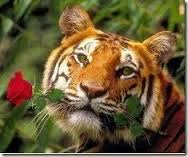
\includegraphics{images/Tiger_Rose.jpg}

\hypertarget{william-carlos-williams}{%
\chapter{William Carlos Williams}\label{william-carlos-williams}}

\hypertarget{the-red-wheelbarrow}{%
\section{The Red Wheelbarrow}\label{the-red-wheelbarrow}}

\begin{quote}
so much depends\\
upon

a red wheel\\
barrow

glazed with rain\\
water

beside the white\\
chickens.
\end{quote}

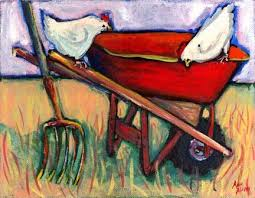
\includegraphics{images/Red_Wheelbarrow.jpg}

\hypertarget{this-is-just-to-say}{%
\section{This Is Just To Say}\label{this-is-just-to-say}}

\begin{quote}
I have eaten\\
the plums\\
that were in\\
the icebox

and which\\
you were probably\\
saving\\
for breakfast

Forgive me\\
they were delicious\\
so sweet\\
and so cold
\end{quote}

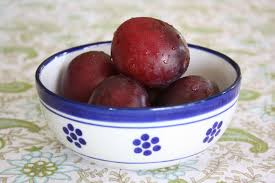
\includegraphics{images/plums.jpg}

\hypertarget{sappho}{%
\chapter{Sappho}\label{sappho}}

\hypertarget{fragment-3-translated-by-julia-dubnoff}{%
\section{fragment 3, translated by Julia Dubnoff}\label{fragment-3-translated-by-julia-dubnoff}}

\begin{quote}
Now, I shall sing these songs\\
Beautifully\\
for my companions.
\end{quote}

\hypertarget{fragment-118}{%
\section{Fragment 118}\label{fragment-118}}

\begin{quote}
Sing, my sacred tortoiseshell lyre\\
come, let my words\\
accompany your voice
\end{quote}

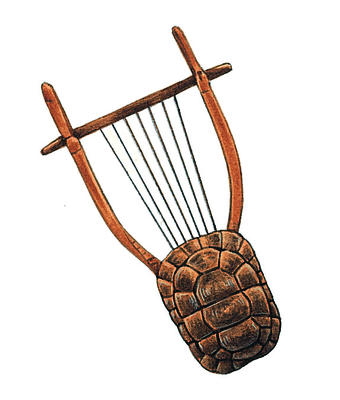
\includegraphics{images/tortoiseshell_lyre.jpg}

\hypertarget{donte-collins}{%
\chapter{Donte Collins}\label{donte-collins}}

\url{https://www.poets.org/poetsorg/poet/donte-collins}

\hypertarget{loving-me-isnt-easy}{%
\section{Loving me isn't easy}\label{loving-me-isnt-easy}}

\begin{quote}
Loving me isn't easy,\\
I have sharp edges,\\
I have missing parts.
\end{quote}

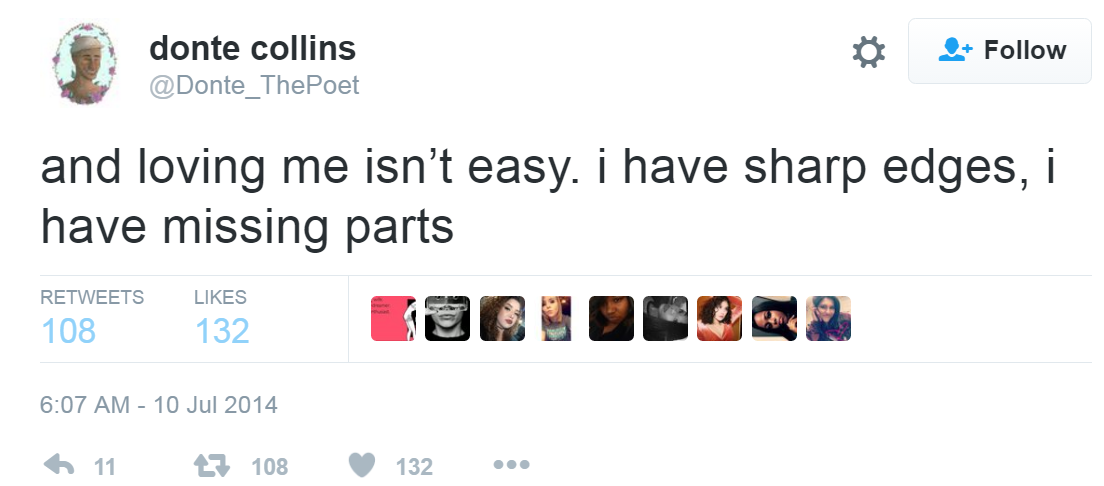
\includegraphics{images/Donte_Collins.png}

\hypertarget{emily-dickinson}{%
\chapter{Emily Dickinson}\label{emily-dickinson}}

\hypertarget{surgeons-must-be-very-careful-156}{%
\section{Surgeons must be very careful (156)}\label{surgeons-must-be-very-careful-156}}

\begin{quote}
Surgeons must be very careful\\
When they take the knife!\\
Underneath their fine incisions\\
Stirs the Culprit---Life!
\end{quote}

\includegraphics{images/.png}

\hypertarget{im-nobody-who-are-you}{%
\section{I'm Nobody! Who Are You?}\label{im-nobody-who-are-you}}

\begin{quote}
I'm nobody! Who are you?\\
Are you nobody, too?\\
Then there's a pair of us - don't tell!\\
They'd banish us, you know.

How dreary to be somebody!\\
How public, like a frog\\
To tell your name the livelong day\\
To an admiring bog!
\end{quote}

\hypertarget{hafiz}{%
\chapter{Hafiz}\label{hafiz}}

\hypertarget{dropping-keys}{%
\section{Dropping Keys}\label{dropping-keys}}

\begin{quote}
\begin{verbatim}
       The small man    
 builds cages for everyone    
      he knows.    
     While the sage,  
 who has to duck his head    
  when the moon is low,  
\end{verbatim}

keeps dropping keys all night long\\
for the beautiful,\\
rowdy\\
prisoners.
\end{quote}

\includegraphics{images/.png}

\hypertarget{conrad-aiken}{%
\chapter{Conrad Aiken}\label{conrad-aiken}}

\hypertarget{bread-and-music}{%
\section{Bread and Music}\label{bread-and-music}}

\begin{quote}
Music I heard with you was more than music,\\
And bread I broke with you was more than bread;
\end{quote}

\includegraphics{images/.png}

\hypertarget{mary-elizabeth-frye}{%
\chapter{Mary Elizabeth Frye}\label{mary-elizabeth-frye}}

\hypertarget{do-not-stand-at-my-grave-and-weep}{%
\section{Do not stand at my grave and weep}\label{do-not-stand-at-my-grave-and-weep}}

\begin{quote}
Do not stand at my grave and weep:\\
I am not there; I do not sleep.\\
I am a thousand winds that blow,\\
I am the diamond glints on snow,\\
I am the sun on ripened grain,\\
I am the gentle autumn rain.\\
When you awaken in the morning's hush\\
I am the swift uplifting rush\\
Of quiet birds in circling flight.\\
I am the soft starshine at night.\\
Do not stand at my grave and cry:\\
I am not there; I did not die.
\end{quote}

\includegraphics{images/.png}

\hypertarget{matsuo-basho}{%
\chapter{Matsuo Basho}\label{matsuo-basho}}

\hypertarget{the-butterfly}{%
\section{The butterfly}\label{the-butterfly}}

\begin{quote}
The butterfly\\
perfuming its wings\\
fans the orchid\\
-translated by Michael R. Burch
\end{quote}

\includegraphics{images/.png}

\hypertarget{takaha-shugyo}{%
\chapter{Takaha Shugyo}\label{takaha-shugyo}}

\hypertarget{fallen-camellias}{%
\section{fallen camellias}\label{fallen-camellias}}

\begin{quote}
Oh, fallen camellias,\\
if I were you,\\
I'd leap into the torrent!\\
-translated by Michael R. Burch
\end{quote}

\includegraphics{images/.png}

\hypertarget{paul-simon}{%
\chapter{Paul Simon}\label{paul-simon}}

\hypertarget{i-am-a-rock}{%
\section{I Am a Rock}\label{i-am-a-rock}}

\url{https://www.youtube.com/watch?v=v_AFN6JuIr8}

\begin{quote}
A winter's day\\
In a deep and dark December;\\
I am alone,\\
Gazing from my window to the streets below\\
On a freshly fallen silent shroud of snow.\\
I am a rock,\\
I am an island.
\end{quote}

\includegraphics{images/.png}

\hypertarget{john-donne}{%
\chapter{John Donne}\label{john-donne}}

\hypertarget{no-man-is-an-island}{%
\section{No Man is an Island}\label{no-man-is-an-island}}

\begin{quote}
No man is an island, entire of itself;\\
every man is a piece of the continent,\\
a part of the main;

if a clod be washed away by the sea,\\
Europe is the less,\\
as well as if a promontory were,\\
as well as any manner of thy friends\\
or of thine own were;

Any man's death diminishes me,\\
because I am involved in mankind.\\
And therefore never send to know\\
for whom the bell tolls;\\
it tolls for thee.
\end{quote}

\includegraphics{images/.png}

\hypertarget{robert-frost}{%
\chapter{Robert Frost}\label{robert-frost}}

\hypertarget{the-dust-of-snow}{%
\section{The Dust of Snow}\label{the-dust-of-snow}}

\begin{quote}
The way a crow\\
Shook down on me\\
The dust of snow\\
From a hemlock tree

Has given my heart\\
A change of mood\\
And saved some part\\
Of a day I had rued.
\end{quote}

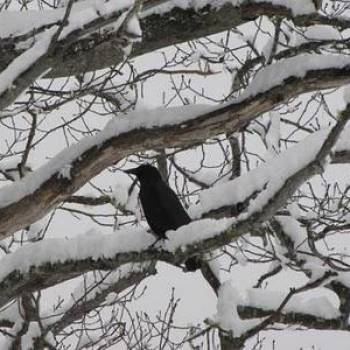
\includegraphics{images/The_Dust_of_Snow.jpg}

\hypertarget{walt-whitman}{%
\chapter{Walt Whitman}\label{walt-whitman}}

\hypertarget{song-of-myself-52}{%
\section{Song of Myself (52)}\label{song-of-myself-52}}

\begin{quote}
You will hardly know who I am or what I mean,\\
But I shall be good health to you nevertheless,\\
And filter and fibre your blood.

Failing to fetch me at first keep encouraged,\\
Missing me one place search another,\\
I stop somewhere waiting for you.
\end{quote}

\includegraphics{images/.png}

\hypertarget{joe-darion}{%
\chapter{Joe Darion}\label{joe-darion}}

\hypertarget{the-impossible-dream}{%
\section{The Impossible Dream}\label{the-impossible-dream}}

\begin{quote}
To dream the impossible dream\\
To fight the unbeatable foe\\
To bear with unbearable sorrow\\
To run where the brave dare not go\\
To right the unrightable wrong\\
To love pure and chaste from afar\\
To try when your arms are too weary\\
To reach the unreachable star

This is my quest\\
To follow that star\\
No matter how hopeless\\
No matter how far

To fight for the right\\
Without question or pause\\
To be willing to march into Hell\\
For a heavenly cause

And I know if I'll only be true\\
To this glorious quest\\
That my heart will lie peaceful and calm\\
When I'm laid to my rest

And the world will be better for this\\
That one man, scorned and covered with scars\\
Still strove with his last ounce of courage\\
To reach the unreachable star
\end{quote}

\href{https://www.youtube.com/watch?v=JjI7VeIA7ZI}{\includegraphics{https://img.youtube.com/vi/JjI7VeIA7ZI/0.jpg}}

\hypertarget{section-55}{%
\section{要做那不可能实现的梦}\label{section-55}}

\begin{quote}
要做那不可能实现的梦,\\
对抗无法匹敌的对手,\\
承受难以承受的悲痛。\\
去往勇者以畏惧之地,\\
纠正那无法改正的错误。\\
成为远远超越自己的人。\\
即使双臂疲惫不堪,\\
仍要尽力去尝试,\\
要摘下那遥不可及的星星。\\
\includegraphics{images/.jpg}
\end{quote}

\hypertarget{edwin-markham}{%
\chapter{Edwin Markham}\label{edwin-markham}}

\hypertarget{the-third-wonder}{%
\section{the Third Wonder}\label{the-third-wonder}}

\begin{quote}
``Two things,'' said Kant, ``fill me with breathless awe:\\
The starry heaven and the moral law!''\\
But I know a thing more awful and obscure---\\
The long, long patience of the plundered poor.
\end{quote}

\hypertarget{section-56}{%
\section{第三奇观}\label{section-56}}

\begin{quote}
有两件事,康德说,会撼动我们的灵魂,\\
一是天上的星空,二是道德的精神,\\
而我知道还有件事,虽然不够明显,\\
但更令人惊心,那就是一无所有的人民,\\
年复一年,怀着巨大的沉默与坚忍。\\
(高观涛译)
\end{quote}

\includegraphics{images/.jpg}

\hypertarget{cahit-sitki-taranci}{%
\chapter{Cahit Sitki Taranci}\label{cahit-sitki-taranci}}

\hypertarget{section-57}{%
\section{火车}\label{section-57}}

\begin{quote}
去什么地方呢?这么晚了,\\
美丽的火车,孤独的火车?\\
凄苦是你汽笛的声音,\\
令人记起了许多事情。

为什么我不该挥手舞手巾呢?\\
乘客多少都跟我有亲。\\
去吧,但愿你一路平安,\\
桥都坚固,隧道都光明。

(余光中译)
\end{quote}

\includegraphics{images/.jpg}

\hypertarget{jacques-prever}{%
\chapter{Jacques Préver}\label{jacques-prever}}

\hypertarget{section-58}{%
\section{一千年一万年}\label{section-58}}

\begin{quote}
一千年一万年\\
也难以诉说尽\\
这瞬间的永恒\\
你吻了我\\
我吻了你\\
在冬日,朦胧的清晨\\
清晨在蒙苏利公园\\
公园在巴黎\\
巴黎是地上一座城\\
地球是天上一颗星

(高行健译)
\end{quote}

\includegraphics{images/.jpg}

\hypertarget{friedrich-holderlin}{%
\chapter{Friedrich Hölderlin(荷尔德林)}\label{friedrich-holderlin}}

\hypertarget{section-59}{%
\section{面包与美酒(第7节)}\label{section-59}}

\begin{quote}
待至英雄们在铁铸的摇篮中长成,\\
勇敢的心象从前一样,\\
去造访万能的神祗。\\
而在此之前,我常感到,\\
与其孤身独涉,不如安然沉睡。\\
何苦如此等待,沉默无言,茫然失措。\\
在这贫困的时代,诗人何为?\\
可是,你却说,诗人是酒神的神圣祭司\\
在神圣的黑夜中,他走遍大地。\\
(刘小枫 译)
\end{quote}

\includegraphics{images/.jpg}

\hypertarget{rilke}{%
\chapter{Rilke(里尔克)}\label{rilke}}

\hypertarget{section-60}{%
\section{秋日}\label{section-60}}

\begin{quote}
主呵,是时候了。夏天盛极一时。\\
把你的阴影置于日晷上,\\
让风吹过牧场。

让枝头最后的果实饱满;\\
再给两天南方的好天气,\\
催它们成熟,把\\
最后的甘甜压进浓酒。

谁此时没有房子,就不必建造,\\
谁此时孤独,就永远孤独,\\
就醒来,读书,写长长的信,\\
在林荫路上不停地\\
徘徊,落叶纷飞。\\
(北岛 译)
\end{quote}

\includegraphics{images/.jpg}

\hypertarget{montale}{%
\chapter{Montale(蒙塔莱)}\label{montale}}

\hypertarget{section-61}{%
\section{生活之恶}\label{section-61}}

\begin{quote}
我时时遭遇\\
生活之恶的侵袭:\\
它似乎喉管被扼断的溪流\\
暗自啜泣,\\
似乎炎炎烈日下\\
枯黄萎缩的败叶,\\
又似乎鸟儿受到致命打击\\
奄奄一息。

我不晓得别的拯救\\
除去清醒的冷漠:\\
它似乎一尊雕像\\
正午时分酣睡朦胧,\\
一朵白云\\
悬挂于清明的蓝天,\\
一只大鹰\\
悠悠地翱翔于苍穹。
\end{quote}

\includegraphics{images/.jpg}

\hypertarget{czesaw-miosz}{%
\chapter{Czesław Miłosz(米沃什)}\label{czesaw-miosz}}

\hypertarget{section-62}{%
\section{恰到好处的一生}\label{section-62}}

\begin{quote}
他的老年遇上富饶的丰收期。\\
没有地震、干旱或洪水。\\
似乎四季的轮转越来越好,\\
星光渐强,太阳增长力量。\\
就连边远的省份也没有打仗。\\
一代代人成长起来,对同胞友善。\\
人的理性本质不是嘲笑的对象。
\end{quote}

\hypertarget{section-63}{%
\section{牧歌}\label{section-63}}

\begin{quote}
微风在园中唤起一阵阵花浪,\\
就像那静谧、柔弱的大海。\\
浪花在绿叶丛中流逝,\\
于是又现出花园和绿色的大海。

翠绿的群山向大河奔去,\\
只有牧童在这里欢歌乐舞。\\
玫瑰花儿绽开了金色的花瓣,\\
给这颗童心带来了欢娱。

花园.我美丽的花园!\\
你走遍天涯也找不到这样的花园。\\
也找不到这样清澈、活泼的流水,\\
也找不到这样的春天和夏天。

这里茂密的青草在向你频频点头,\\
当苹果滚落在草地上时,\\
你会用你的目光跟踪它,\\
你会用你的脸庞亲昵它。

花园,我美丽的花园!\\
你走遍天涯也找不到这样的花园,\\
也找不到这样清澈、活泼的流水,\\
也找不到这样的春天和夏天。
\end{quote}

\includegraphics{images/.jpg}

\hypertarget{nadine-stair}{%
\chapter{Nadine Stair}\label{nadine-stair}}

\hypertarget{id-pick-more-daisies}{%
\section{I'd Pick More Daisies}\label{id-pick-more-daisies}}

\begin{quote}
If I had my life to live over,\\
I'd try to make more mistakes next time.\\
I would relax. I would limber up.\\
I would be sillier than I have on this trip.\\
I would be crazier. I would be less hygienic.\\
I would take more chances, I would take more trips.\\
I would climb more mountains, swim more rivers,\\
and watch more sunsets.\\
I would burn more gasoline. I would eat more ice cream and less beans.\\
I would have more actual troubles and fewer imaginary ones.\\
You see, I am one of those people who lives\\
prophylactically and sensibly and sanely,\\
hour after hour, day after day.

\begin{verbatim}
           Oh, I have had my moments  
\end{verbatim}

And if I had it to do over again, I'd have more of them.\\
In fact, I'd try to have nothing else.\\
Just moments,one after another.\\
Instead of living so many years ahead each day.\\
I have been one of those people who never go anywhere\\
without a thermometer, a hot water bottle, a gargle, a\\
raincoat, and a parachute.

\begin{verbatim}
If I had to do it over again, I would go places and do things.  
                   I'd travel lighter than I have.  
  If I had my life to live over, I would start barefooted  
     earlier in the spring and stay that way later in the fall.  
       I would play hooky more. I wouldn't make such good grades  
            except by accident.  
               I would ride on merry-go-rounds.  

                    I'd pick more daisies!  
\end{verbatim}
\end{quote}

\hypertarget{section-64}{%
\section{我会采更多的雏菊}\label{section-64}}

\begin{quote}
如果我能够从头活过,\\
我会试着犯更多的错。

我会放松一点,我会灵活一点。\\
我会比这一趟过得傻。\\
很少有什么事情能让我当真。

我会疯狂一些,我会少讲点卫生。\\
我会冒更多的险。我会更经常的旅行。\\
我会爬更多的山,游更多的河,看更多的日落。\\
我会多吃冰激凌,少吃豆子。\\
我会惹更多的麻烦,可是不在想象中担忧。

你看,我小心翼翼地稳健地理智地活着。\\
一个又一个小时,一天又一天。

噢,我有过难忘的时刻。\\
如果我能够重来一次,我会要更多这样的时刻。

事实上,我不需要别的什么,\\
仅仅是时刻,一个接着一个。\\
而不是每天都操心着以后的漫长日子。

我曾经不论到哪里都不忘记带上:\\
温度计,热水壶,雨衣和降落伞。

如果我能够重来一次,\\
我会到处走走,什么都试试,并且轻装上阵。\\
如果我能够重头活过,\\
我会延长打赤脚的时光。\\
从尽早的春天到尽晚的秋天。

我会更经常的逃学。\\
我不会考那么高的分数,除非是一不小心。\\
我会多骑些旋转木马,\\
我会采更多的雏菊。
\end{quote}

\hypertarget{robert-penn-warren}{%
\chapter{Robert Penn Warren(罗伯特·潘·沃伦)}\label{robert-penn-warren}}

\hypertarget{section-65}{%
\section{我一路走来}\label{section-65}}

\begin{quote}
我一路走来,\\
坐在树影里,\\
膝上放着书,但一无所思。\\
我凝视着\\
小儿子在下午的阳光中嬉戏。

痉挛,吵闹\\
夜起伏呼吸,燃烧,而星星\\
陨落。我记得什么?\\
我听见沼地的枭鹰整夜呼唤,\\
而远处汽车的前灯扫过房间。

我是个阴暗狡黠的家伙,\\
我从阴影里朝外看,\\
你一绺绺头发闪着阳光,\\
我看着你在阳光下嬉戏,\\
儿子,请你教我白昼的方式。\\
(赵毅衡译)
\end{quote}

\hypertarget{ways-of-day}{%
\section{WAYS OF DAY}\label{ways-of-day}}

\begin{quote}
I have come all this way.\\
I am sitting in the shade.\\
Book on knee and mind on nothing,\\
I now fix my gaze\\
On my small son playing in the afternoon's blaze.

Convulsive and cantankerous,\\
Night heaved, and burning, the star\\
Fell. What do I remember?\\
I heard the swamp owl, night-long, call.\\
The far car's headlight swept the room wall.

I am the dark and tricky one.\\
I am watching from my shade.\\
Your tousled hair-tips prickle the sunlight.\\
I watch you at your sunlit play.\\
Teach me, my son, the ways of day.
\end{quote}

\hypertarget{section-66}{%
\section{世事沧桑话鸣鸟}\label{section-66}}

\begin{quote}
那只是一只鸟在晚上鸣叫,认不出是什么鸟,\\
当我从泉边取水回来,走过满是石头的牧场,\\
我站得那么静,头上的天空和水桶里的天空一样静。

多少年过去,多少地方多少脸都淡漠了,有的人已谢世,\\
而我站在远方,夜那么静,我终于肯定\\
我最怀念的,不是那些终将消逝的东西, 而是鸟鸣时那种宁静。\\
(赵毅衡 译)
\end{quote}

\hypertarget{ornithology-in-a-world-of-flux}{%
\section{Ornithology in a World of Flux}\label{ornithology-in-a-world-of-flux}}

\begin{quote}
It was only a bird call at evening, unidentified,\\
As I came from the spring with water, across the rocky back-pasture;\\
But so still I stood sky above was not stiller than sky in pail-water.

Years pass, all places and faces fade, some people have died,\\
And I stand in a far land, the evening still, and am at last sure\\
That I miss more that stillness at bird-call than some things\\
that were to fail later.
\end{quote}

\hypertarget{minecraft}{%
\chapter{Minecraft}\label{minecraft}}

\hypertarget{my-name-is-steve-a-short-minecraft-story-for-the-curious}{%
\section{MY NAME IS STEVE: A short Minecraft story for the curious}\label{my-name-is-steve-a-short-minecraft-story-for-the-curious}}

Don't ask me what I'm doing here, because I don't know. One day, I woke up in the middle of a forest, covered in snow, devoid of all memory and sense of identity. Why? I have no clue. It almost doesn't matter.

I spent the first couple of hours calling for help, wandering around, hoping I'd find someone nearby. After a while, I came to the reluctant conclusion that I was well and truly isolated: no sound of human voices, no hum of tires on distant roadways; nothing but the trill of far off birds and rustling branches in the wind. There might have been a cow nearby from all the mooing, but I couldn't find it.

I might not have known who I am, or why I woke up in this snowy forest, but that didn't mean I was going to sit down and let depression take me along with the wolves. I needed a plan of action, needed to find a way to survive! But first, a man needs to know himself before he can trust himself, and because my old name was lost to my departed memory, I have decided to call myself Steve.

It's a good name.

I spent some time searching the area, looking for anything that might be useful to me. Tools and weapons would be my first priority--don't ask me how I knew, but I could tell the forest would be dangerous at night, something in my blood maybe. There wasn't much, not even a single fallen branch on the ground, just smooth snow and straight pine trees. I tried to grab hold of a few rocks peeking up from the soil, but they were firmly stuck. I'd need something to pry them free, or maybe break them away. I spotted a tree nearby and went to it, running my hands over the dark brown bark. It was a good tree, strong and healthy.

So I punched it.

Pulp and bark flew as my hard fists broke chunk after chunk away from the tree. I gritted my teeth against the jarring in my arms and kept going until the whole thing broke through and crashed to the ground. Chest heaving from the exertion, I gathered the wood and sat down, examining the pieces. I broke some of the longer chunks into thick sticks, then stabbed one of them into a flat piece of wood shaped like a blade.

I grinned as I hefted the wooden axe I'd made, then swung it around experimentally. It felt good. I used the axe to fell several more trees until I had enough wood to make all the tools I needed: a shovel, sword, and pickax--the latter of which I used to break those stubborn stones from the ground. I stowed the rocks away for later use and strapped the tools to my back. I kept the sword out though, the feeling of danger in the woods tickling the back of my mind. Thus armed, I set off in search of food and shelter.

I won't bore you with the details of my struggle against starvation and wolves. Suffice it to say, it was a struggle. I fought, bled, and conquered. I stumbled over hills and down into water-filled valleys, climbing trees to see the path ahead. I slew cows and ate their flesh to stay alive. I fell off cliffs and broke bones, spending days waiting for them to heal. I briefly marveled at how quickly the wounds mended, but wasted no time in pressing on once they did. At night times, I was attacked by monsters, proving my intuition about the forest to be correct. I hid from the darkness, lighting the small mud huts I'd built along the way with torches until the sun rose once again.

I never knew why the world I'd woken up in was filled with skeletons and zombies, but it didn't really matter, I bashed their heads in with stone swords nonetheless. There were more questions to be had than answers, and I knew I would never know the half of them.

I had to survive!

Weeks later, exhausted, clothes ripped and torn, blood from numerous cuts on my legs trailing into my socks, I finally found mountains. Majestic. I climbed them each, looking for the ideal spot to build a home, far away from the oppressive trees and monster-filled shadows of the forest.

I avoided the caves beneath those mountains, fearful of skeletons and massive spiders. I knew I would have to venture inside them eventually, but not then. I finally found a flat-topped peak that overlooked the forests to the east, and ocean to the west. From its heights, I would be able to see the whole land, and defend my homestead from intruders. It was good.

That was a few months ago. I've since become used to this way of life, in this strange land. The name of Steve fits me like a glove, and I am the master of my modest stone home. I've raised cattle, planted wheat, and baked bread. I've explored those mysterious caves and returned the victor, bringing home coal for fires, iron for tools and armor, precious gold and even a priceless diamond. I am king of all I see, master of this forsaken land.

And then yesterday, my house blew up. Not all of it, but a good chunk of the western corner. You see, I was up on the roof, placing some wooden shingles that had blown loose in a rain storm, when a creeper appeared from of nowhere. I tried to pull back out of sight, but he spotted me and exploded in a fit of suicidal rage.

Now, I might not have mentioned creepers before, but not because they don't bear describing.

I call them creepers, because that's what they do. I first discovered them while exploring my first cave, and let me tell you: damn. Those things are scary as all hell. On that first instance, I'd run out of torches, and was blindly trying to feel my way forward, stone sword at the ready, when a movement caught my eye. I backed away, stumbling into the light of my torches, my head filled with thoughts of spiders and zombies, but instead\ldots{} something else emerged, creeping along the stone with four stubby legs attached to a long torso. Its face stared at me with a strange sadness, mouth gaping in a profound grimace, arm stumps wiggling uselessly at its shoulders.

I stared, horrified by this hideous beast, lulled into apathy with misplaced pity.

But when the creeper neared, I caught a whiff of gunpowder, and the cave filled with an ominous hissing. I came to my senses and tried to flee as the hissing reached a crescendo. The creeper writhed and pulsed, its mouth opening in agony only a split second before it exploded in a roar of fire and flying rock. I threw myself down, covering my head with my arms as flames billowed over me.

I almost died that day, and learned to fear the creeper above all others.

And so, my house in smoking splinters after the latest creeper attack, I knew I had to repair it quickly before night fell and I became easy meat for monsters. I stowed all my valuables in a chest and armed myself with seven stone axes and iron armor, prepared to gather as much wood as possible before nightfall. I headed down to the edges of the forest and spent all day felling trees, breaking their wood into rough chunks I could carry back.

But somehow during the hours spent sweating and breaking axes, I got lost.

As the sun turned orange and dipped toward the horizon, I knew I had to get to shelter--fast. These lands bred monsters, and the sun's rapid progress worried me. With nothing but my axes and the wooden boards I'd hewn, I dug a hole in the ground and prepared to wait out the night.

But before I finished plugging up the entrance, I was spotted.

Spiders!

I put the last board in place and listened with dread in the dark as a dozen clacking mandibles drooled at the thought of my sweet blood just overhead. Their filthy mouths squealed and their clawed legs thumped all around as they did a frenzied, pre-meal dance, waiting for me to emerge. I slept uneasily in the dirt, listening to the terrible sounds above. When the morning came, they were still there. I cleared my bleary eyes and fashioned a crude sword from some stone beneath my feet and wood from my pockets, vowing to at least go down with a fight.

With a deep breath, I broke through the wooden barrier and leapt to the offense!

``My name is STEEEEEVE!'' I screamed in defiance, but there were too many!

I ducked and dodged, keeping my lightly armored limbs from the six spiders' poisoned fangs as I hacked at their hairy bodies. But they pressed in.

I tried to retreat, but my foot fell into the very hole I'd hidden in overnight, and I tripped. I landed heavily in the dirt, gazing at the patch of sunlight above through my pain. Somehow, I knew this was the sky I would die under. I thought about the cows in their pens, the sheep grazing peacefully by the golden wheat ready to be harvested. They would all wait forever for me to return. My house would remain on my mountain top, an empty monument to Steve, the only human to ever walk this world. Was it all for nothing? No.~I'd survived, if only for a while.

I blinked and brought myself back to the present. I smiled grimly as the spiders tried to swarm into the small hole, but their disgusting bodies were too big. I hacked at them from below, killing several. Perhaps there was a chance--

My hope was short lived, and my stomach dropped as a creeper suddenly appeared, blindly following the spiders, hoping for an easy victim. How could my luck have been so horrible? I knew what was going to happen next. Adrenaline flashed through my veins and I threw myself back as the creeper toppled into the hole, coming to land in a heap not two feet from me. I was trapped! The cold dirt and unyielding stone pressed against my back as I turned away, squeezing my eyes shut as the dreaded sound filled the small hole\ldots.

sssssssSSSSSSSS\ldots.

One day, I woke up in the middle of a forest, covered in snow\ldots.

THE END
\textgreater{}

\includegraphics{images/.jpg}

\backmatter
\backmatter
\printindex

\end{document}
